\documentclass{article}
\usepackage[utf8]{inputenc}
\usepackage{graphicx}
\usepackage{hyperref}
\usepackage{geometry}
\geometry{a4paper} % Set the page size to A4
\usepackage{listings} % Package for including code in the document

\title{Práctica 07: Funciones en SQL}
\author{Carlos I. Padilla Herrera}
\date{13 de mayo de 2024}

\lstset{frame=single, % Adds a frame around the code
        basicstyle=\small\ttfamily, % Use a small, true type font
        language=SQL, % SQL syntax highlighting
        showstringspaces=false} % Don't mark spaces in strings

\begin{document}

\begin{titlepage}
    \centering
    \vspace*{1cm}
    \Huge\textbf{Curso de base de datos entre semana G0224}
    
    \vspace{0.5cm}
    \LARGE Escuela de Código PILARES
    
    \vspace{1.5cm}
    \textbf{Carlos Ignacio Padilla Herrera}
    
    \vspace{2cm}
    \Large\textbf{Folio:} 794DR02
    
    \vspace{0.5cm}
    \Large\textbf{Práctica 08:} Disparadores.
    
    \vfill
    
    \Large\textbf{Fecha:} 13 de mayo de 2024.
    
    \vspace{0.8cm}
\end{titlepage}

\newpage

\section*{Código SQL para la creación de la base de datos y la tabla}

\begin{lstlisting}
    create database if not exists test;
    use test;
    
    create table alumnos (
        id int unsigned auto_increment primary key,
        nombre varchar(50),
        apellido1 varchar(50),
        apellido2 varchar(50),
        nota float
    );    
\end{lstlisting}
\begin{figure}[ht]
    \centering
    {
        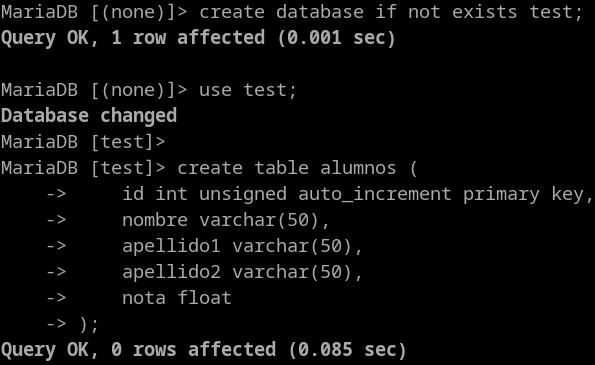
\includegraphics[width=\linewidth]{01screenshot.png} % Asegúrate de que el nombre del archivo y la extensión son correctos
    }
    \caption{Captura de pantalla de la creación de la base de datos y la tabla.}
\end{figure}
\newpage % Inicia una nueva página

\section*{Código del disparador (trigger) para operaciones de inserción.}

\begin{lstlisting}
    delimiter //
create trigger trigger_check_nota_before_insert
before insert on alumnos
for each row
begin
    if new.nota < 0 then
        set new.nota = 0;
    elseif new.nota > 10 then
        set new.nota = 10;
    end if;
end;
//
delimiter ;
\end{lstlisting}

\begin{figure}[ht]
    \centering
    {
        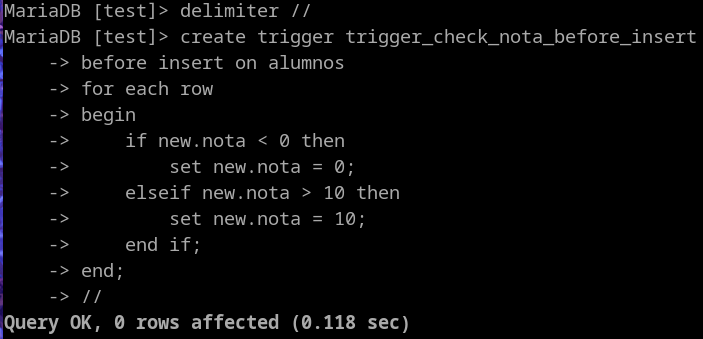
\includegraphics[width=\linewidth]{02screenshot.png} % Asegúrate de que el nombre del archivo y la extensión son correctos
    }
    \caption{Captura de pantalla del disparador para operaciones de inserción.}
\end{figure}

\newpage % Inicia una nueva página

\section*{Disparador 2 para operaciones de actualización}

\begin{lstlisting}
    delimiter //
create trigger trigger_check_nota_before_update
before update on alumnos
for each row
begin
    if new.nota < 0 then
        set new.nota = 0;
    elseif new.nota > 10 then
        set new.nota = 10;
    end if;
end;
//
delimiter ;
\end{lstlisting}
\begin{figure}[ht]
    \centering
    {
        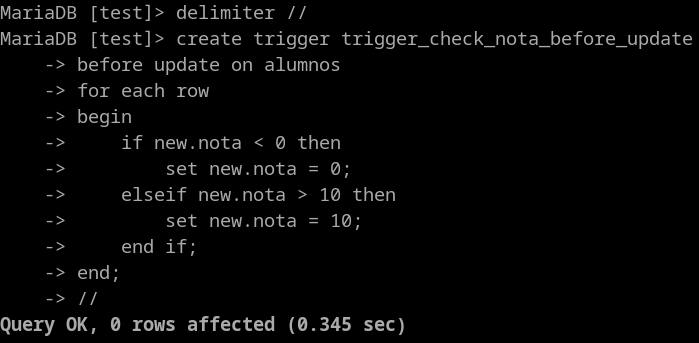
\includegraphics[width=\linewidth]{03screenshot.png} % Asegúrate de que el nombre del archivo y la extensión son correctos
    }
    \caption{Captura de pantalla del disparador de operaciones de actualización.}
\end{figure}

\newpage % Inicia una nueva página

\section*{Sentencias de inserción y actualización para probar los disparadores}
\begin{lstlisting}
	insert into alumnos (nombre & apellido1 & apellido2 & nota) 
    values (`juan' & `perez' & `lopez' & -3); \\
	insert into alumnos (nombre & apellido1 & apellido2 & nota) 
    values (`laura' & `garcia' & `morales' & 12); \\
	insert into alumnos (nombre & apellido1 & apellido2 & nota) 
    values (`carlos' & `sanchez' & `gomez' & 8); \\
\end{lstlisting}
\begin{figure}[ht]
    \centering
    {
        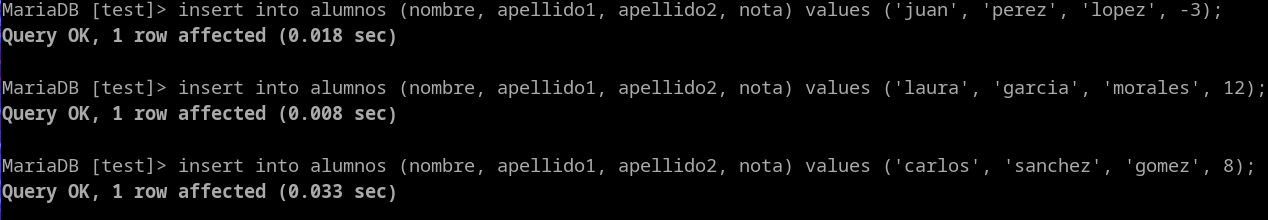
\includegraphics[width=\linewidth]{04screenshot.png} % Asegúrate de que el nombre del archivo y la extensión son correctos
    }
    \caption{Captura de pantalla de las sentencias de inserción en la base de datos.}
\end{figure}

\newpage % Inicia una nueva página

\section*{Sentencias de actualización}
\begin{lstlisting}
    update alumnos set nota = 15 where nombre = 'carlos';
    update alumnos set nota = -1 where nombre = 'laura';
\end{lstlisting}
\begin{figure}[ht]
    \centering
    {
        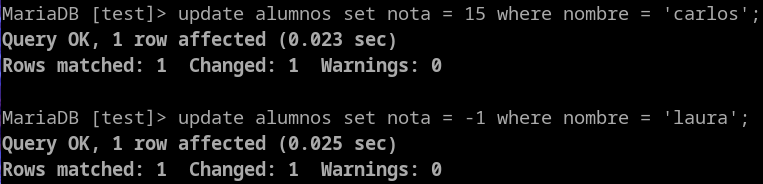
\includegraphics[width=\linewidth]{05screenshot.png} % Asegúrate de que el nombre del archivo y la extensión son correctos
    }
    \caption{Captura de pantalla de las sentencias de actualización.}
\end{figure}

\section{Verificar que los disparadores están funcionando como se espera con la siguiente consulta.}
\begin{lstlisting}
    select * from alumnos;
\end{lstlisting}

\begin{figure}[ht]
    \centering
    {
        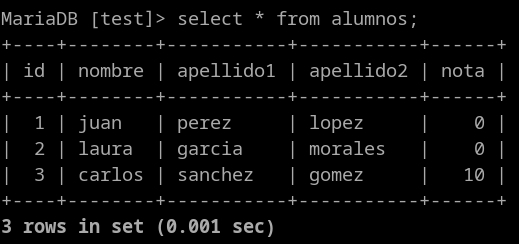
\includegraphics[width=\linewidth]{06screenshot.png} % Asegúrate de que el nombre del archivo y la extensión son correctos
    }
    \caption{Captura de pantalla que comprueba que los disparadores funcionan como se espera.}
\end{figure}
\newpage % Inicia una nueva página

\end{document}
